%chapter_cacop_begin
\graphicspath{ {../body/cacop_figures/}}
\chapter{基于多媒体特性的呼叫接纳控制算法研究}
\label{chap_cacop}

从目前无线网络的发展情况看,多媒体数据业务将会逐渐取代目前无线通信中话音业务为主的状况。
为此,无线通信标准中的定义中已经开始支持这些多媒体业务的传输。例如,IEEE802.16定义了多媒体数据的调度类型。
本章首先研究和提出针对不同业务类型服务质量的归一化定义。
然后根据这一定义提出了以系统服务质量最优的呼叫接纳控制原则及其相应的接纳控制算法。

\section{前言}
呼叫接纳控制本质是一个管理呼叫连接并进行资源分配与管理的技术。
这项技术以往常常在无线话音网络,如GSM网络,或VoIP(Voice over Internet Protocol)的网络中使用\cite{Perros1996}\cite{Mase2004}。
有时,它也会应用到视频通信的网络中,用来保证连接的视频质量\cite{Systems_2001}\cite{Y-G-Fang.TVT.2002}\cite{Y-Xiao.IEICE.TC.2001}。
通常,它也被看作是在有限的无线频谱资源与大量的资源需求之间的折衷的策略。
比如,在电话服务网络中,由于业务对数据延时的敏感性,使得呼叫接纳控制单元,为了避免网络数据的拥塞不得不拒绝一些连接的接入。
如果在这些情况下不采取相应的措施,网络的状况会发生拥塞甚至恶化。
另外,呼叫接入控制还间接影响着网络资源的分配与管理。
例如,当某一个连接的数据流过于贪婪,占用了大量的网络资源时,
它会造成其它连接的业务服务质量下降,使得网络不得不阻塞新的连接进入或是导致现有连接的中断。
这都将使得网络服务的用户的满意度下降。

近此年来,研究人员提出许多呼叫接纳控制的算法或方案。
有些算法是根据基本的网络性能参数直接用来建立呼叫接纳的准则。这此参数包括比如带宽资源利用率、单位时间内的数据包的个数或在线的呼叫个数等。
当这些参数的值达到或超过了预先设置的上限或是下限,新的呼叫将会被迫延迟接入或是拒绝接入\cite{Y-Qian.TWC.2006} \cite{G-Djuka.TELSIK.2007}。
还有些是将一些底层(物理层或MAC层)的参数加以合并建立基于交叉层的新准则来应用来呼叫接纳控制算法。
例如,学者Song和Zhuang引入了一个被称之SRPT(shortest remaining processing time)的服务准则 \cite{Song2009}。
一个时间窗的大小被设置到一个合适的阈值来判断连接或呼叫是否被接入网络。
学者Yilmaz 和 Chen 也提出了一个类似的思想\cite{Yilmax2009}.
在这篇文献中,他们将资源标上价格并设置价格的阈值。
这种竞价方案是通过分析一个或多个数据流的特点来完成。
最后提出的接纳控制方案使用一个或是多个混合分区的价格阈值,并且周期地对资源进行定价来使系统的效用最大化。
那些不能负担资源费用的用户会被系统拒绝服务。
学者Zhai和Ni提出一个半马尔可夫决策过程来描述呼叫接纳过程 \cite{Zhai2005,Ni2009}。
他们通过把呼叫过程转化为一个求解系统资源利用最大化的数学问题。
学者Zhai和Xiang提出一个信道繁忙率(channel busyness ratio)的概念。
通过检测信道繁忙率来为呼叫接纳提供判断的准则 \cite{Zhai_Chen_Fang_2006}。
还有的学者是通过资源预留的方法来解决呼叫接纳的问题。
例如,Chen和Kuo提出通过动态指派优先级的方法来接纳呼叫 \cite{Chen_Kumar_Kuo_2003,Chen_Kuo_2004}。
学者Elsayed等将三种比例预留的策略:统一预留、容量比例预留和剩余比例预留做了详细的评估\cite{Elsayed02performanceevaluation}。
学者El-Kadi提出的动态预留的方法 \cite{EL-Kadi2002}。
这种方法引入用户数据在短时间内可以容忍通信质量一定程度上的下降,并且基于此提出“借和还”的比例预留方法。
此方法与我们将在本章提出的方法有些类似,所以本章仿真实验中当作对比实验。

以往的这些接纳控制方案中所涉及的测量参数大多都集中在物理层和MAC层上,很少从用户应用的角度来思考呼叫接纳控制。
这主要有两个原因:一个是以前的无线网络承载的业务基本上以话音为绝大多数。其它的业务量极小。
二是尽管可以用交叉层技术使得网络底层得到上层如应用层的流量信息,但是这样会破坏无线网络的分层结构。
所以交叉层技术的应用范围局限性较大。
因此要寻求其它的途径来完成这一任务。
本章的贡献就在于此。
本章首先构造一个简单的服务质量评估模型,将应用层信息与底层参数信息做一个适当的映射关系。
然后,将此模型应用于接纳控制及资源分配,可以在兼顾资源利用效率的情况下,又可保证终端用户所感受到的服务质量。
%
\section{MAC层业务调度类型分类}
随着网络业务的发展,无线通信标准也开始关注业务的种类对通信质量的影响。
譬如,在WiMAX(Worldwide Interoperability for Microwave Access)中,
标准的制定者对MAC层数据包做了初步的分类。
他们把数据分为五类:
每一类业务类型有自己相应的服务质量参数,例如延迟、抖动、丢包或错包率等等。
每一类数据的调度算法都应尽可能满足这些服务质量参数\cite{Tsagkaris_Demestichas_2009}\cite{Andrews_Ghosh_Muhamed_2007}。
%但是同时,我们也注意到WiMAX的标准仅仅将这些数据分类而已,并没有说明如何调度这些已经分类的数据。这也给学者留下一块研究的空间。
此处我们也参照着WiMAX标准定义,将业务分成以下几类。

\begin{itemize}
\item UGS( unsolicited grant service)业务:这种业务类型是指具有实时性要求的业务。
    它的数据具有是周期性产生、包长固定的特点。
    比如T1、E1以及没有静默压缩的VOIP等就属于此类业务。
    这个特点使得UGS业务的数据流比较稳定,突发性较差。
\item rtPS(real-time polling services)业务:这类业务也是具有实时性要求,
    但是与UGS业务不同,它的数据包一般是变长的,同时也具有周期性。
    这类数据包的包头也比UGS数据包的包头要大。
    例如象MPEG(Motion Pictures Experts Group)视频或H.264视频流。
    在调度此类数据时,采用基站指导下移动台单播轮询策略(unicast polling)。
    基站需要通过提供足够多的轮询次数来保证业务的实时性要求。
\item nrtPS (non-real-time polling services)业务:
    这种业务与rtPS业务十分类似。但是它采用的是移动台竞争轮询策略(contention-based polling)。
    如果在竞争轮询期间此类用户很多,就会出现资源申请冲突和后续的冲突避让方案。
    所以,这种方式会引入较大的时间延迟。
\item BE (best-effort)业务:
    此类业务对服务质量的要求在五种业务类型中最低。往往也没有十分具体的QoS指标要求。
    如果能够申请到资源,就进行数据发送。如果不能,则继续等待下一次的调度。
    一般我们把普通的文字网页浏览,或是FTP文件的传送归于此类。
\item ertPS(extended real-time polling service)业务:
    这种业务类型是将上行数据链路的传输协议做了复用。
    在传数据的同时,也可进行无线资源的申请。
    这样可以保证数据量波动较大的情况下,资源能够得到及时的调度。
\end{itemize}

\section{呼叫接纳控制模型与业务流的QoS分析}
\label{sec_qos_metric}
因为不同的业务数据对服务质量的要求差别很大,所以要设计相应的传输机制来应对这种变化。
本节我们将详细描述如何将接纳控制方案与资源分配方案相结合。

%CAC
\subsection{呼叫接纳控制模型}
\label{sec_sec_model}
前面我们提到,呼叫接纳控制的方案就是为了避免网络拥塞,决策某一个呼叫或连接通信服务是否被中断或拒绝。
(因为呼叫一般专指话音通信,所以为避免文字概念混淆,下文一律用“连接”一词来代替“呼叫”一词。)
此处,我们假设一个一般的呼叫接纳控制的网络模型。
在此模型中,有一个基站和~$K$~连接,如\figref{fig_system_model_cac}所示。

其中包括已经在线的$K-1$个连接和$1$个正在申请进入的新连接。
这些连接根据不同的业务种类被分为五种类型,UGS,rtPS,nrtPS,BE和ertPS。
在第$K$个连接被接入之前,所有 ($K-1$) 连接共享基站所提供的带宽资源,记为$B_{total}$。
当第$K$个连接进入基站的覆盖范围,并提交进入和资源分配的申请后,系统触发一次接纳控制的判断过程。
首先,服务质量评估单元(QoS Evaluator)会根据目前的连接情况,提交一份带宽资源分配的方案,记为向量 $\mathbf{b}$ 。
其中,$b_i$ 表示第$i$个连接所分配到的带宽,那么,$\mathbf{b} = [ b_1, b_2, b_3, \dots, b_K]$ ,而且 $\sum_{i=1}^K b_i \le B_{total}$。
然后,
基于这个方案 $\mathbf{b}$,接纳控制单元(Call Admission Control)根据每一个连接所分配到的带宽 $b_i$来评估每一个连接的QoS水平和整个系统的QoS水平。
最后,接纳控制单元再决定接受或拒绝这个连接的进入请求。
%%
\begin{figure*}[t]
\centering
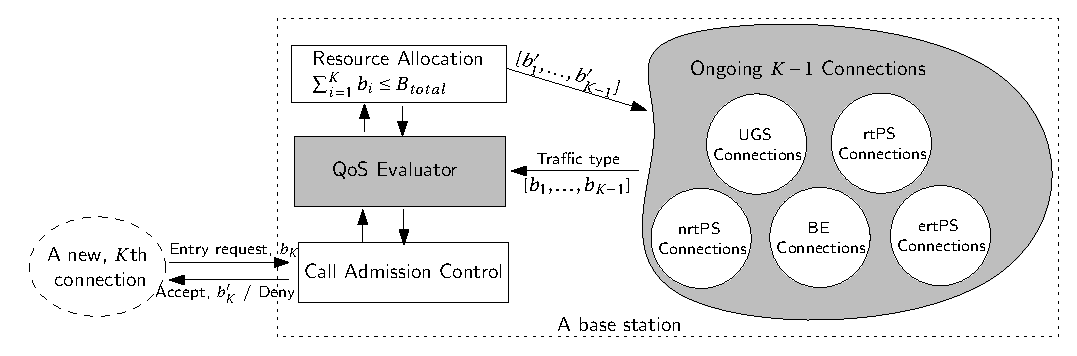
\includegraphics[width=0.95\textwidth]{cac_qos_model_system.eps}
\caption{ 呼叫接纳控制的系统模型} \label{fig_system_model_cac}
\end{figure*}
%%%%%%
%QoS Metric
\subsection{QoS Metric and Bandwidth Allocation}





























































\iffalse
在无线网络资源管理中,呼叫接纳控制(CAC,Call admission control)对于服务质量(QoS,Quality of service)起着十分重要的作用。在本章中,我们首先根据视频流的特性,引入一个可以应用在呼入控制中的新的QoS测量方法。通过这个新的测量方法可以更加有效地利用无线网络的带宽资源。对于一个高负荷的网络,可以理论证明,如果使用了这个测量方法,存在一个优化的带宽分配方案。这个方案在保持各个连接服务质量的同时,可以最大化基站系统的QoS效用。最后,我们通过模拟实验来验证和评估这个呼叫接纳控制的方法。实验的结果表明,这个方案可在资源利用率与用户的QoS水平之间取得更好的平衡。

\section{引言}
\label{section_cacop_introduction}
\par 呼叫接纳控制的本质是通过管理或限制用户的接入请求数目进入网络来达到减轻网络拥塞的一种方法。
这种方法通常会与资源分配与数据流量调整紧密相关。也可看做是一种在有限的网络资源与大量的用户资源要求之间的一种折衷方案\cite{Y-G-Fang.TVT.2002} \cite{Y-Xiao.IEICE.TC.2001}。例如,在传统的电话网络中,呼叫接纳控制在网络拥塞的情况下会拒绝用户的接入请求,而不是让过多用户直接参与无线网络的资源共享。因为与Internet的普通数据业务不同,话音业务是一种实时的通信业务。它对数据的延时十分敏感。超过延时门限的数据包将会被丢弃。所以,如果不采用适当的接入控制技术,过多的网络流量与网络请求会对用户的服务质量造成损害,进而引起用户的不满意度上升。另一个方面,接入控制技术也要处理另一个资源管理的问题,网络资源分配的公平性。如果某一个用户数据流过多的占用了网络的带宽,那么同样会带来请求接入的用户被拒绝服务或是在线的用户掉线。同样会引起用户的满意度下降和网络资源利用率的效用下降。
\par 为此,许多学者在过去的许多年里,对无线接入控制技术做了大量的研究,并提出了一些新型的接入控制算法\cite{Y-Qian.TWC.2006} \cite{G-Djuka.TELSIK.2007}。他们中的大部分首先建立一个系统的效用模型,然后基于这个模型建立一个服务阈值,从而对接入的用户进行判断。例如,学者Song和Zhang引入一个称为最短剩余处理时间的服务准则(SRPT,the shortest remaining processing time),然后再设置一个合适的阈值来判断用户是否可以被接入 \cite{Song2009}。学者Yilmaz和Chen也提出了一个类似的方案。他们的工作首先分析了在多个数据流与单个数据流的接入控制的特点,提出了一个通过竞价来确定阈值的接入控制方案。这个方案需要周期地更新价格来最大化系统的收益。如果在竞价中失败或是不能支付资源最终价格的用户或是连接会被拒绝服务 \cite{Yilmax2009}。在文献 \cite{Zhai2005,Ni2009},他们的工作是通过建立一个半马尔可夫决策过程(SMDP, the semi-Markov decision process),把接入控制问题转化成一个数学上的资源利用率的最大化问题。另外一些学者方法,是通过采取折衷的方案来处理接入控制问题。这些方案允许接入的用户的资源请求数量被大部分的满足,服务质量可以少量下降,但不会引起用户的不满意度上升。例如,学者El-Kadi等人提出了一个临时租借资源的方法来处理资源不足的问题。对于一个新到来用户,它可以通过向已经在线的用户租借资源的方式来达到自己请求资源的要求。租借资源的量是与用户的服务质量的最低容忍度为极限的 \cite{EL-Kadi2002}。
\par 这些接入控制方案都不没有考虑到数据流本身的特性。在本章中,我们首先引入了一个用来评价视频流数据服务质量的评测参数。依据这个参数,建立一个无线网络基站的效用模型;然后通过这个模型来处理接入控制问题。

\section{CAC的调度模型}
为了不失一般性,这里我们考虑一个通常的无线通信的接入模型,如图 \ref{  fig:cacop_system_model_cac}。这个模型包括一个基站控制器和$K$个数据流的用户连接。其中,有$K-1$个在线用户的连接和一个新的正在请求接入的用户连接。这些连接共享所有的带宽资源~$B_{total}$。当一个用户进入基站的信号覆盖范围时,发出自己的带宽请求。CAC控制器根据此时自身的带宽资源状态和用户状态,执行一个CAC的算法得到一个资源分配的向量~$\mathbf{b}$,其中,$b_i$是分配给第$i$个用户连接的带宽资源。则有,
$$\mathbf{b} = [ b_1, b_2, b_3, \dots, b_K]$$
$$\sum_{i=1}^K b_i \le B_{total}$$.
根据资源分配向量~$\mathbf{b}$,我们在进一步考查每个连接的QoS水平来决定它是否被拒绝服务。

%%%%%%%%%%%%%%%%%%%%%%%%%%%%%%%%%%%%%%%%%%%%%%%%%%%%%%%%%%%%%%%%%%%%%
\begin{figure}[tb]
\begin{centering}
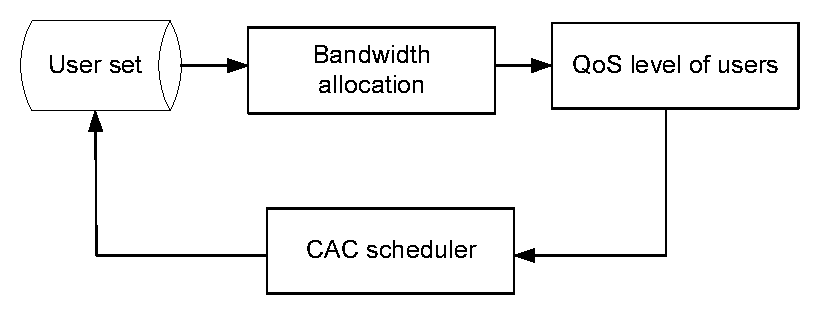
\includegraphics[scale=0.7]{../figures/cacop_system_model_cac}
\caption{CAC的调度模型示意图}
\label{ fig:cacop_system_model_cac }
\end{centering}
\end{figure}
%%%%%%%%%%%%%%%%%%%%%%%%%%%%%%%%%%%%%%%%%%%%%%%%%%%%%%%%%%%%%%%%%%%%%

\section{QoS的测量与带宽分配}
一个CAC的算法的本质是决定在系统中的哪些用户的数据连接被继续保持服务状态或是被拒绝服务,进而可以避免网络拥塞状况的出现。大部分的CAC算法可以归纳成优化的问题。它们通过测量物理层(如信号的强度)或是数据链路层的参数(数据包的延迟),然后根据这些参数来优化系统的效用。与它们的优化参数不同,我们的方法侧重于视频用户的应用层的QoS参数。通过视频编码中的率失真优化策略(RDO, rate distortion optimization)来设计一个便于可以在数据链路层使用的QoS的测量方法。我们可以证明基于这种测量方法的CAC算法,可以将基站系统效用最优化。这种方法的优点在于,可以仅通过请求的带宽数据,不用获取上层的数据就可以达到较为精确的估计。从而与一般意义的交叉层优化需要直接从上层得到应用层的信息不同,这种方法可以适用于更一般的网络,因而适用性更广。
\section{数据链路层上视频流的QoS水平的度量}
在视频的实际应用和学术研究中,普遍采用的是一种名为峰值信噪比(PSNR, Peak signal-to-noise ratio )的参数。它是一种流行的视频质量客观评价的标准。它本质是同一幅图像处理前后图像的差。PSNR的定义是通过均方误差(MSE)来定义的。对于尺寸为 MxN 图像I与图像K来说,PSNR数学定义如下:
\begin{equation}
PSNR = \frac{10 \log (2^n -1)^2 }{ MSE }
\end{equation}

\begin{equation}
MSE = \frac{1}{MN} \sum^{M-1}_{x=0} \sum^{N-1}_{y=0} \left[ I(x,y) - K(x,y) \right] ^2
\end{equation}
其中,$n$是每一个象素点的采样比特数。通常对于视频的压缩,一般的视频应用的PSNR的值在30到50dB。对于无线网络的传输,这个指标有时也可放宽到20dB到25dB。
然而,PSNR这个参数却不能够直接应用于呼叫控制中的用户或连接的QoS水平的度量。首先,这要求视频流需要被解码才能还原为原始的压缩前的图像,对于基站而言,这是不现实的。其次,PSNR的计算要求提前知道原始的参考图像才能计算,在实际的传输过程中,基站的CAC控制器无法得到这些视频数据,所以也不可能计算得到这些值。对于基站而言,它只能得到一些关于带宽的需求和用户的类型之类的信息。所以,通常的QoS测量的做法是度量网络的吞吐量,将一个用户已经得到带宽资源与要求的带宽资源的比值做为一个QoS的度量。例如,对于用户$i$,基站分配给它的带宽信息是$b_i$, 它想要的带宽是$B_i$,那么这个QoS的测量公式可定义为
\begin{equation}
QoS_i = \frac{b_i}{B_i}
\end{equation}
这个方法对于普通的网络应用如HTTP或是FTP是适用的。因为它们对于数据带宽的可以认为是线性的。而对于视频应用而言,这种线性关系通常是不满足的。所以,本章我们引入一个新的方法来度量用户的QoS。它和PSNR类似但又适用于呼叫接纳控制。我们发现,率失真优化技术(RDO, Rate distortion optimization)可能利用并应用在我们的CAC控制中。RDO技术在视频编码过程中,通过建立起视频的码率与失真之间的近似关系来进行优化编码的技术。这种方法,也建立起了视频QoS测量与CAC带宽分配之间的关系。通常RDO的关系,失真与码率之间大多是一种e指数关系。\cite{E-H-Yang.TIP.2007} \cite{J-Y-Liu.ICIP.2009} \cite{He1013856} 根据这种关系,我们提出了一个公式(\ref{eqn:qos_level_users})来定义视频质量与带宽分配之间的关系。
%%%
\begin{equation}
\alpha = \frac{1- e^{-\rho \frac{b}{B} }}{1-e^{-\rho}},
\label{eqn:qos_level_users}
\end{equation}
%%%
这里,我们用$\alpha$来表示一个视频流的质量,$1- e^{-\rho \frac{b}{B}},\rho \ge 1$表示视频的QoS水平,分母${1-e^{-\rho}}$表示归一化系数。小写字母$b$表示视频流可以分配到的带宽资源,这个值通常要求要大于最小带宽要求$B_{min}$,大写字母$B$表示这个视频流所想要申请到的资源。为了进一步校验这个式子,我们编码了一些标准视频测试序列与公式\ref{eqn:qos_level_users}相比较,如图\ref{fig_qos_rate_cac}。正如所期望的那样,所提出的这个公式可以较好的做为视频流的QoS的一个估计。因此,我们也可用它来做为视频流的QoS水平与视频分配带宽之间的一个关系。
%%%%%%
\begin{figure}[tb]
\begin{center}
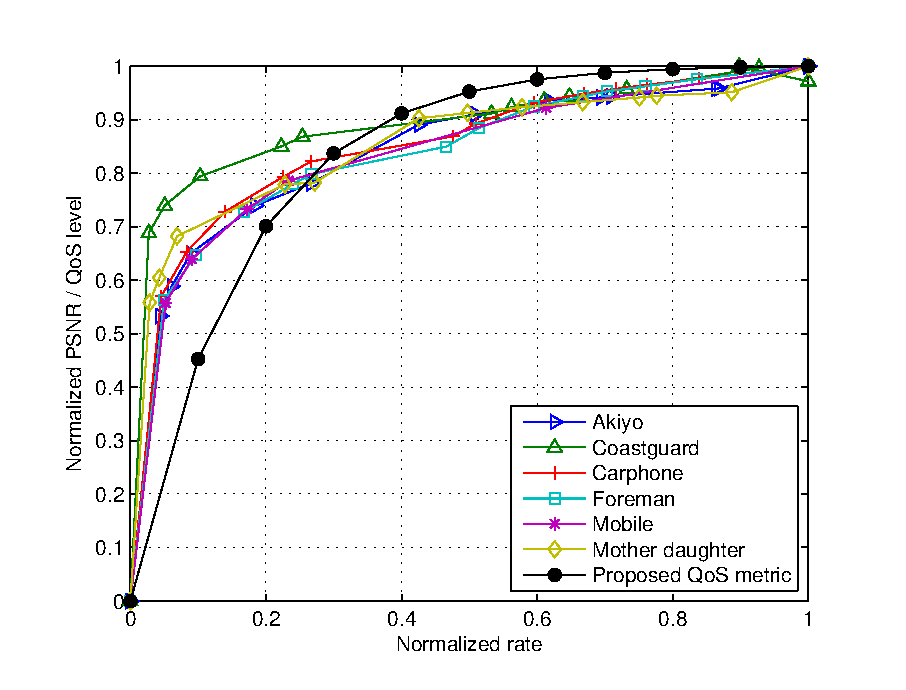
\includegraphics[scale=0.7] {qos_rate_cac.eps}
\end{center}
\caption{所提出的视频流QoS的与归一化的PSNR之间的比较,其中视频流为 Akiyo, Coastguard, Carphone, Foreman, Mobile, 和 Mother\&daughter. } 
\label{fig_qos_rate_cac}
\end{figure}
%%%%%%

\subsection{优化的资源分配方案}
因为呼入控制的目的是为了在系统带宽容量一定的情况下,尽可能的满足用户的需要,所以我们构造了一个优化问题。又因为QoS的计算每个用户都是独立的,所以我们将所有连接的QoS水平加起来,做为我们优化的目标,如公式(\ref{eqn:bs_qos})所示。
%%%
\begin{eqnarray}
U_{BS} &=& \displaystyle \sum_{i=1}^K \alpha_i \nonumber \\
&=&\displaystyle \sum_{i=1}^K \left( \frac{1- e^{-\rho
\frac{b_i}{B_i} }}{1-e^{-\rho}} \right) ,\label{eqn:bs_qos}
\end{eqnarray}
%%%
其中,$U_{BS}$表示当BS要给$K$个用户提供服务时,整个BS的效用。为了最大化$U_{BS}$,我们要为这些视频用户找到一个带宽分配的最优解$\mathbf{b}$。然后,根据这个解来进一步判断哪一个连接或用户会被拒绝服务。这个优化问题,被定义为如下:
%%%
\begin{eqnarray}{}
\mathbf{b}^* &=& \arg \max \left\{ U_{BS}(\mathbf{b}) \big| \mathbf{b} = [b_1, b_2, \dots, b_K] \right\} \label{eqn_u_bs_qos}\\
& &\text{subject to:}\nonumber\\
& &\displaystyle\sum_{i=1}^{K}b_i + B_{ava}= B_{total} \nonumber
\end{eqnarray}
%%%
这里,$\mathbf{b}$是一个带宽分配的优化的解,$B_{total}$是BS所能提供的全部带宽资源。$B_{ava}$是所有的可用的带宽资源。我们在此处做如下的假设,在一个系统负荷较大的情况下,$B_{ava}$为零。那么,CAC的方案就是为了解决系统资源不足的情况下,如何更好分配资源。
%
\vspace{5mm}{
\theorem 如果带宽分配问题被定义为如公式(\ref{eqn_u_bs_qos})所示,那么就一定存在一个资源分配方案 ~$\mathbf{b}^*$ 使得系统的效用~ $U_{BS}$ 达到最大。
}\vspace{3mm}

\proof
为了证明简单起见,我们先引入一个临时的变量~$x_i$,并定义如下。
%%%
\begin{equation*}
\begin{split}
x_i = \frac{b_i}{B_i}.
\end{split}
\end{equation*}
%%%
%
然后,我们根据拉格朗日乘数法,引入拉格朗日乘子~$\lambda$。则拉格朗日方程可以写为如下公式。
%%%
\begin{equation}
\begin{split}
F (x_1, x_2, x_3, \dots, x_K, \lambda) = \sum^K_{i=1}
\left( \frac{1-e^{-\rho x_i}}{1-e^{-\rho}} \right) \\+ \lambda
\left(B_{total} - \sum^K_{i=1} x_i B_i \right).
\end{split}
\end{equation}
%%%
对方程求偏导数 $\frac{\partial ^2F}{\partial x_i \partial x_j}$,可得 Hermitian 矩阵 $M$。

%%%
\begin{eqnarray*}
{M} = & 
\left[
\begin{array}{ccccc}
\frac{\partial ^2F}{\partial x_1 ^2} &\frac{\partial ^2F}{\partial x_1 \partial x_2} & \dotsi & \frac{\partial ^2F}{\partial x_1 \partial x_{K-1}}& \frac{\partial ^2F}{\partial x_1 \partial x_K} \\
\frac{\partial ^2F}{\partial x_2 \partial x_1}& \frac{\partial ^2F}{\partial x_2 ^2}& \dotsi & \frac{\partial ^2F}{\partial x_2 \partial x_{K-1}}&\frac{\partial ^2F}{\partial x_2 \partial x_K}\\
\vdots & \vdots & \ddots & \vdots & \vdots \\
\frac{\partial ^2F}{\partial x_{K-1} \partial x_1 } &\frac{\partial ^2F}{\partial x_{K-1} \partial x_2}&\dotsi &\frac{\partial ^2F}{\partial x_{K-1}^2}&\frac{\partial ^2F}{\partial x_{K-1} \partial x_K}\\
\frac{\partial ^2F}{\partial x_{K} \partial x_1 } &\frac{\partial ^2F}{\partial x_{K} \partial x_2} & \dotsi & \frac{\partial ^2F}{\partial x_{K} \partial x_{K-1}}&\frac{\partial ^2F}{\partial x_K ^2}\\
\end{array}
\right] \\
=&
\left[
\begin{array}{ccccc}
\frac{-\rho^2 e^{-\rho x_1}}{(1-e^{-\rho})} \\
&\frac{-\rho^2 e^{-\rho x_2}}{(1-e^{-\rho})} & & \text{{\huge{0}}}\\
& &\ddots\\
& \text{{\huge{0}}} & & \frac{-\rho^2 e^{-\rho x_{K-1}}}{(1-e^{-\rho})}\\
& & & &\frac{-\rho^2 e^{-\rho x_K}}{(1-e^{-\rho})}
\end{array}
\right] 
\end{eqnarray*}
因为$\rho \ge 1, x_i \ge 0$,所以,矩阵$M$是负定的矩阵。所以,对于$U_{BS}$而言,存在一个带宽分配的方案,使得$U_{BS}$取到最大值。

接下来,我们来求解这个带宽分配的优化方案。首先,我们对公式()求偏导数,可得下面一系列的式子。
%%%
\begin{subequations}
\label{eqn_derivate}
\begin{align} &\frac{\partial F}{\partial x_1} =
\frac{\rho e^{-\rho x_1}}{(1-e^{-\rho})} - \lambda B_1 = 0 \tag{\theequation -1}\\
&\frac{\partial F}{\partial x_2} =
\frac{\rho e^{-\rho x_2}}{(1-e^{-\rho})} - \lambda B_2 = 0 \tag{\theequation -2}\\
\nonumber & \qquad \vdots \qquad \vdots \qquad \vdots \\
&\frac{\partial F}{\partial x_K} =
\frac{\rho e^{-\rho x_K}}{(1-e^{-\rho})} - \lambda B_K = 0 \tag{\theequation -K}\\
&\frac{\partial F}{\partial \lambda} = B_{total} -
\sum^K_{i=1}x_iB_i = 0 \tag{\theequation -K+1}
\end{align}
\end{subequations}
%%%
根据公式 (\ref{eqn_derivate}-1), 我们可得

%%%
\begin{equation*}
\begin{split}
&\frac{\partial F}{\partial x_1} = \frac{\rho e^{-\rho
x_1}}{(1-e^{-\rho})} - \lambda B_1 = 0\\
\implies &\rho e^{-\rho x_1} =\lambda B_1(1-e^{-\rho})\\
%\implies &e^{-\rho x_1} = \frac{tB_i(1-e^{-\rho})}{\rho} \\
\implies &-\rho x_1 = \ln \left[\lambda B_1(1-e^{-\rho}) \right] -
\ln \rho \\
\implies &x_1 = -\frac{1}{\rho} \ln \left[
\lambda B_1(1-e^{-\rho})\right] + \frac{1}{\rho} \ln \rho \\
\implies &x_1 = -\frac{1}{\rho}\ln \lambda - \frac{1}{\rho} \ln
(B_1) - \frac{1}{\rho}\ln (1-e^{-\rho}) + \frac{1}{\rho} \ln
\rho
\end{split}
\end{equation*}
%%%

%%%
根据上面类似的推导过程,我们可以得到下面的结果。
%%%
\begin{equation*}
\begin{split}
x_2 &= -\frac{1}{\rho}\ln \lambda - \frac{1}{\rho} \ln (B_2) -
\frac{1}{\rho} \ln (1-e^{-\rho}) + \frac{1}{\rho} \ln
\rho \\
x_3 &=-\frac{1}{\rho} \ln \lambda- \frac{1}{\rho} \ln (B_3) -
\frac{1}{\rho} \ln (1-e^{-\rho}) + \frac{1}{\rho} \ln
\rho\\
\nonumber &\vdots \qquad \vdots \qquad \vdots \\
x_K &=-\frac{1}{\rho} \ln \lambda- \frac{1}{\rho} \ln (B_K) -
\frac{1}{\rho} \ln (1-e^{-\rho}) + \frac{1}{\rho} \ln \rho
\end{split}
\end{equation*}
%%%
然后,我们将$x_i$代入(\ref{eqn_derivate}-K+1),可得
%%%
\begin{equation}
\begin{split}
&B_{total} = \sum_{i=1}^K x_i B_i \\
&= \sum^K_{i=1}\left[- \frac{1}{\rho}\ln \lambda - \frac{1}{\rho}
\ln (B_i) - \frac{1}{\rho} \ln (1-e^{-\rho}) + \frac{1}{\rho}
\ln
\rho \right] B_i\\
&= \sum^K_{i=1}\left[- \frac{B_i}{\rho} \ln \lambda -
\frac{B_i}{\rho} \ln (B_i) - \frac{B_i}{\rho} \ln (1-e^{-\rho})
+ \frac{B_i}{\rho} \ln
\rho \right]\\
&= -\frac{\ln \lambda}{\rho} \sum^K_{i=1} B_i - \frac{1}{\rho}
\sum^K_{i=1} B_i \ln (B_i)- \frac{\ln(1-e^{-\rho})}{\rho}
\sum_{i=1}^K B_i \\ & \hspace{5mm}+ \frac{ \ln \rho} {\rho} \sum^K_{i=1} B_i
\end{split}
\label{eqn_find_mu}
\end{equation}
%%%
基于公式(\ref{eqn_find_mu}),我们可以求得$\lambda$
%%%
\begin{equation*}
\begin{split}
\lambda &= \exp \left( \frac{-\rho B_{total} - \sum^K_{i=1} B_i \ln
(B_i) }{\sum^K_{i=1}B_i} \right.\\
&+ \left. \frac{ - \ln(1-e^{-\rho}) \sum^K_{i=1}B_i + \ln \rho
\sum^K_{i=1}B_i}{\sum^K_{i=1}B_i} \right)\\
&= \exp \left( \frac{-\rho B_{total} - \sum^K_{i=1} B_i \ln
(B_i) }{\sum^K_{i=1}B_i} - \ln(1-e^{-\rho}) + \ln \rho \right)
\end{split}
\end{equation*}
%%%

然后,又可得
%%%
\begin{equation}
\begin{split}
x_i &=-\frac{1}{\rho} \ln \lambda- \frac{1}{\rho} \ln (B_i) -
\frac{1}{\rho} \ln (1-e^{-\rho}) + \frac{1}{\rho} \ln \rho
\\
&= \frac{\rho B_{total} + \sum^K_{k=1}B_k ln (B_kK) + \ln(1 -
e^{-\rho} )\sum^K_{k=1}B_k - \ln \rho \sum^K_{k=1}
B_k)}{\rho \sum^K_{k=1}B_k} \\&\quad - \frac{1}{\rho} \ln B_i
-\frac{1}{\rho} \ln(1-e^{-\rho}) + \frac{\ln \rho}{\rho}
\\
&= \frac{B_{total}}{\sum^K_{k=1}B_k} + \frac{\sum^K_{k=1}B_k
\ln (B_k)}{\rho \sum^K_{k=1}B_k} + \frac{1}{\rho}
\ln(1-e^{-\rho}) - \frac{\ln \rho}{\rho} \\
& \quad - \frac{1}{\rho} \ln B_i -\frac{1}{\rho}
\ln(1-e^{-\rho}) + \frac{\ln \rho}{\rho} \\
& = \frac{B_{total}}{\sum^K_{k=1}B_k} +\frac{\sum^K_{k=1}B_k \ln
(B_k)}{\rho \sum^K_{k=1}B_k} - \frac{1}{\rho} \ln B_i
\end{split}
\end{equation}
%%%
最后,资源分配方案的解为:
\begin{equation}
\begin{split}
b_i^* &= x_i B_i \\
&= \frac{B_i B_{total}}{\sum^K_{k=1}B_k} +\frac{B_i \sum^K_{k=1}B_k
\ln (B_k)}{\rho \sum^K_{k=1}B_k} \\&\quad - \frac{B_i \ln
B_i}{\rho}, \quad i=1,2,\dots,K
\end{split}
\label{eqn:b_i_bw}
\end{equation}
所以,我们可以下结论说,根据上述的推导过程,我们有唯一的解对应于资源的分配方案~$\mathbf{b}$。

\section{提出的CAC方案}
\label{sec_cacop_alg}
这里我们提出一种简单的CAC方案。这个方案是基于上一节中的带宽资源的分配方案。这个方案的流程显示如流程图 \ref{agr_cac}。当一个新的用户进入基站的覆盖范围,它发出请求接入请求。随后,接入控制过程开始。如果此时,基站的资源比较宽松,可用的资源大于这个用户(标记为用户K)的请求,那么毫无疑问它会立刻被允许接入。如果基站的可用资源十分紧张,则CAC控制器会计算这个用户的最优带宽的分配值$b_K^*$。如果这个值大于这个用户所能容忍的最小资源需求,那么这个用户的接入申请仍会被接受。反之,这个用户的接入申请会被拒绝。假设这个用户被允许接入,那么接下来,在线的$K-1$个用户要调整它们的目前使用的资源使得整个基站系统的效用最大。然后,这个新用户会分配资源$b_K^*$。这样的方法,将可以总能保持整个系统的效用最大化。

%%%%%
% CAC scheme explanation
\begin{algorithm}[bt]
%\SetAlgoLined
%  assume $B_{ava}=0$\;
等待一个新的用户请求\;
第~$K$个用户发出进入基站服务的请求,所需的带宽资源为~$B_K$,假设此时在基站系统中正在接收服务的用户有~$K-1$\;
\eIf {$B_K<= B_{ava}$}{
接受这个新用户进入请求,根据它的带宽请求,并分配资源~$B_K$给它\;
}{
根据公式(\ref{eqn:b_i_bw})计算其可以得到的带宽资源的优化值~$b_K^*$  \;
\eIf{$b_K< B_K^{min}$}{
    拒绝这个用户的进入请求\;
    {\bf{go to 1}}\;
}{
  接受这个用户的请求,\;
 \For{$i=1$ \KwTo $K-1$}{
根据公式(\ref{eqn:b_i_bw})计算求得第~$i$个用户的带宽资源的分配值 \;
 Allocate $b_i^*$ to the $i$th connection\;
}
并分配给新用户~$b_K^*$的带宽资源\;
}
}
{\bf{转到第1步}}\;
\caption{所提出的新CAC方案}
\label{agr_cac}
\end{algorithm}

\section{仿真实验与结果}
\label{cacop_sim}
%%%%%%%%
%
\begin{figure}[tb]
\centering
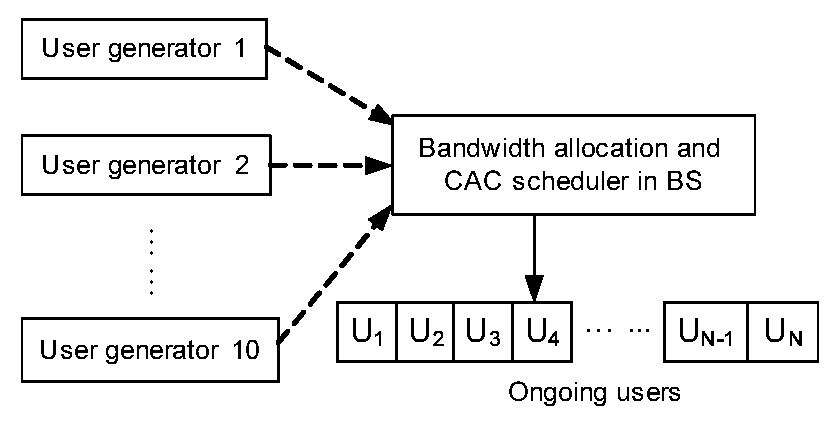
\includegraphics[width=3in] {simulator.eps}
\caption{Simulation configuration} \label{pic_cacop_sim_cfg}
\end{figure}

为了简单起见,我们通过一个简化的基站服务仿真模型来评估我们提出的CAC方案,如图\ref{pic_cacop_sim_cfg}。在这个模型中,设置了十个用户接入申请发生器和一个基站CAC控制器。这些用户接入申请发生器发送接入申请到基站CAC控制器。这些申请是按照Poisson模型,速率$r=30 \text{ to } 100 $每小时。它们在基站接受服务的时间服从指数分布,其中均值为 600 到 1500 秒。带宽请求值从600Kbps到2Mbps。详细的参数见表格 \ref{tb_cacop_sim_cfg}。基站控制器负责接受用户的接入申请,并执行一个CAC的方案来决断是否接入这个申请,并分配和调整用户的资源大小。全部可用的带宽为75Mbps。

同时,我们选择了其它二种CAC的方案做为实验中的对比方案。一种方案叫Baseline。这种方案中,CAC控制器依照简单的接入原则。如果目前系统中可用的带宽大于用户的需求带宽,那么就允许接入。反之,则拒绝这个用户。另一种对比方案ElKadi采用了的按比例资源拆借方案。如果用户请求的资源比系统中可用的空闲资源多,那么就把所有的在线用户的资源减少一个固定的比例,放入空闲资源池中。从而满足新的申请用户的带宽资源需要。\cite{EL-Kadi2002} 这个方案其实也是一种资源预留的方案。

表格 \ref{tb_cacop_res_sim} 显示了这三种CAC方案的仿真的统计结果。我们比较了传统的网络参数如在线用户数、带宽的利用率;也比较了本章中提出的QoS的参数。可以从表格中的数据可以看出,我们提出的方案比其它两个方案的综合性能要好。例如,Eldadi方案的带宽利用率最低,但是同时它的用户的请求拒绝率表现最好。对于Baseline方案而言,它通过大量地拒绝新用户的请求来保证在线的用户的QoS。与这二者相对应的,我们的方案可以做出较好的折衷,在基本保持接通率的情况下,增加带宽的利用率。对用基站系统的效用可以保持在141.4,而单个用户的QoS保持在0.984(最大值为1)。
图\ref{cacop_pic_clock_accept_block_drop} - \ref{cacop_pic_clock_avg_call_qos}分别显示了这三种方法在各种评价参数的仿真曲线。Elkadi的方法的带宽利用率曲线的波动情况比其它两种方法要大,如图\ref{cacop_pic_clock_bs_availble_bw}所示。这是因为这种方法通过降低在线服务的用户的所使用的资源而对新用户做了资源的预留。这样做优点是显著提高新用户的接入率。而且,在线用户的数目也会较多,如图\ref{cacop_pic_clock_onging_call_sum}所示。这种方法却在QoS上牺牲了在线用户的QoS,明显,平均QoS曲线,在三种方法中它是最低的。Baseline的方法会使得用户平均QoS曲线总是保持为最大。它是通过拒绝大量的新的用户来保证这一点。这样做也明显对新的用户不太公平。无论是Elkadi方法还是Baseline方法,都不能在资源受限的情况下做出较好的折衷。但是,我们提出的方法可以保持平均QoS比Elkadi方法高,同时,用户接入的拒绝率与带宽利用率都可以平衡的较好。

\begin{table}[tb]
\caption{仿真中用户连接的类型} \label{tb_sim_cfg}
\begin{center}
\def\temptablewidth{1\textwidth}
{\rule{\temptablewidth}{1pt}}
\begin{tabular*}{\temptablewidth}{@{\extracolsep{\fill}}cccc}
请求的带宽资源 & 最低的带宽需求 &到达率 &在基站中停留的时间 \\
(Kbps) & (Kbps) & (/hour) &(seconds) \\
\hline
 64 &64 & 100 &600\\
90 &64 &90 &700\\
128 &64 &80 &800\\
256 &128 &70 &900\\
384 &192 &60 &1000\\
768 &384 &50 &1100\\
1024 &512 &40 &1200\\
1512 &756 &40 &1200\\
1768 &884 &30 &1500\\
2048 &1024 &30 &1500\\ \hline
\end{tabular*}
 {\rule{\temptablewidth}{1pt}}
 \end{center}
 \end{table}

\begin{table}[tb]
\caption{仿真的结果统计} \label{tb_cacop_res_sim}
\begin{center}
\def\temptablewidth{1\textwidth}
{\rule{\temptablewidth}{1pt}}
\begin{tabular*}{\temptablewidth}{@{\extracolsep{\fill}}llll}
 &Baseline &Elkadi &Proposed\\
\hline
拒绝率 (\%) &14.8 & 1.2 &4.0\\
用户的连接平均个数&128.0 &146.5 &142.7\\
基站的QoS水平 &128.0 &140.6 &141.4\\
单个用户的平均QoS水平 &1.00 &0.960 &0.984\\
带宽利用率(\%) &95.6 &87.8 &93.8\\
%Block rate (\%) &14.8 & 1.2 &4.0\\
%Connection capacity &128.0 &146.5 &142.7\\
%QoS level of BS &128.0 &140.6 &141.4\\
%Avg. QoS level of connections &1.00 &0.960 &0.984\\
%Bandwidth utilization(\%) &95.6 &87.8 &93.8\\
 \hline
\end{tabular*}
 {\rule{\temptablewidth}{1pt}}
 \end{center}
\end{table}

%%%%%%%
%
\begin{figure}[htb]
\centering
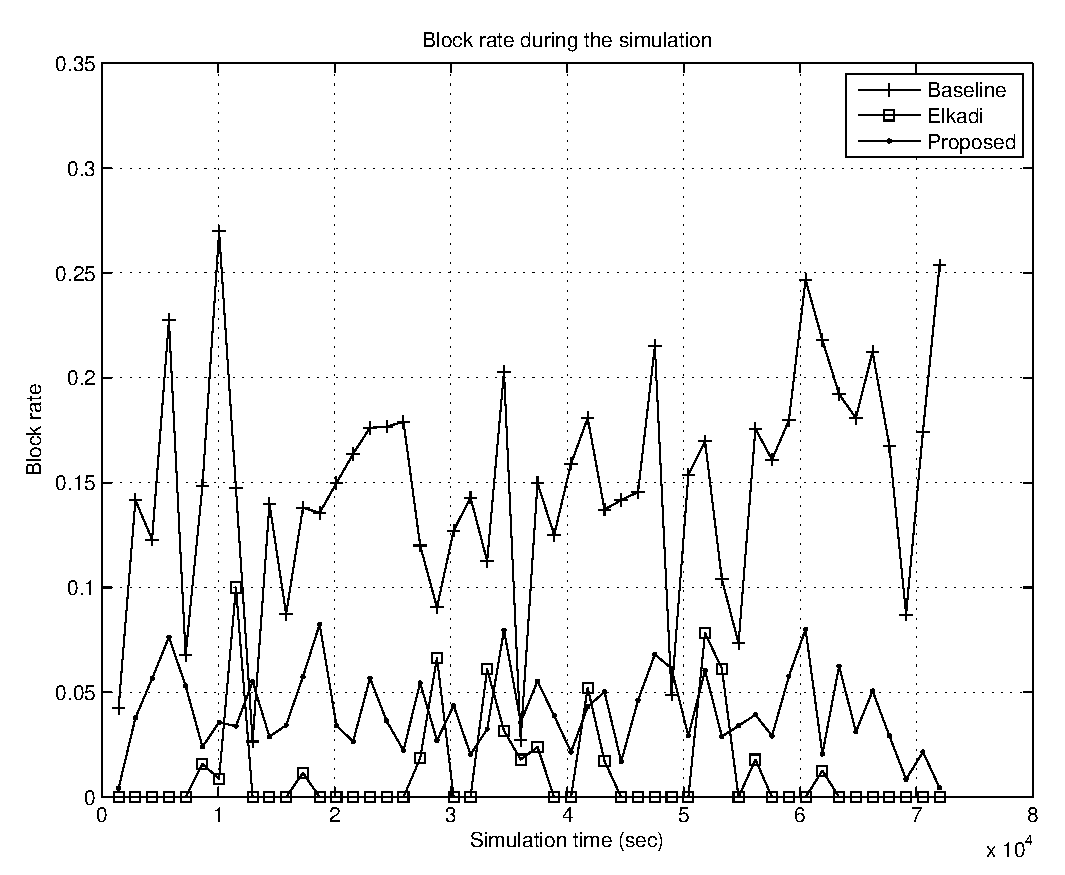
\includegraphics[width=4in] {clock_accept_block_drop.eps}
\caption{基站中用户请求接入的拒绝率}
%\caption{Comparison of block rate of connections in a BS}
\label{cacop_pic_clock_accept_block_drop}
\end{figure}

%%%%%%%
%
\begin{figure}[htb]
\centering
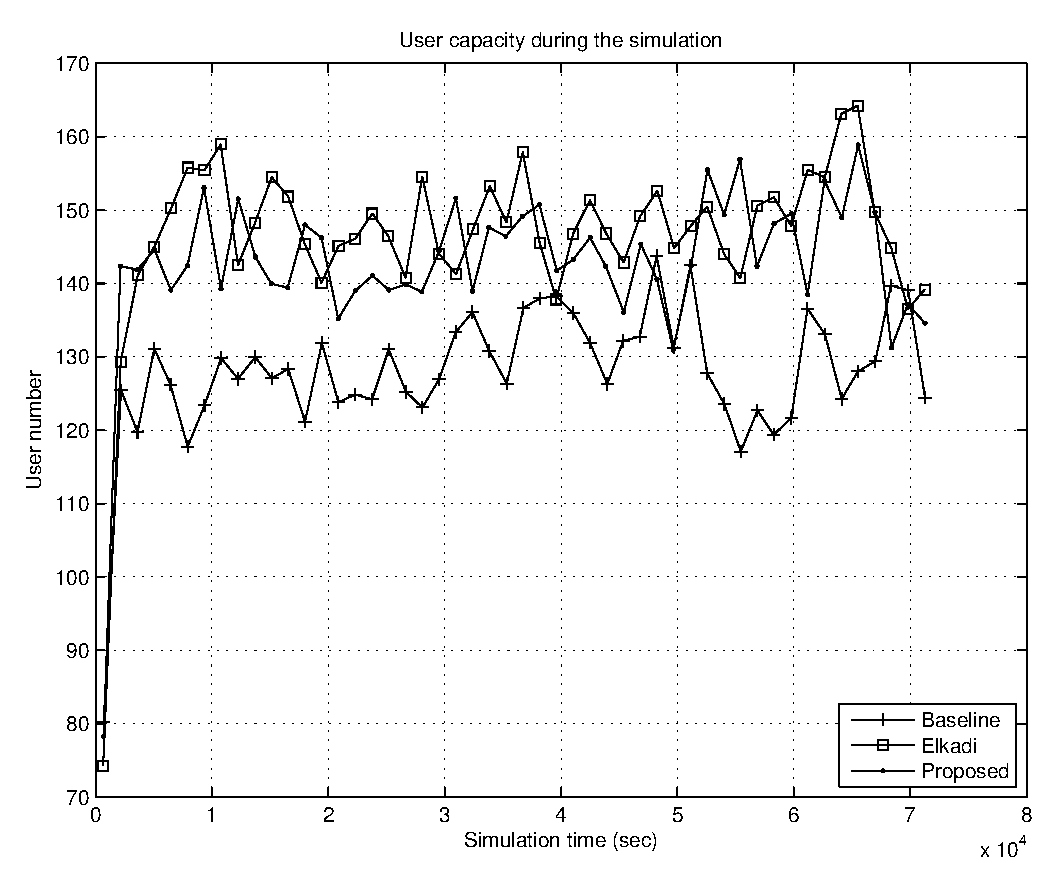
\includegraphics[width=4in] {clock_onging_call_sum.eps}
\caption{基站的在线用户数}\label{cacop_pic_clock_onging_call_sum}
%\caption{Comparison of number of connections in a BS}\label{cacop_pic_clock_onging_call_sum}
\end{figure}

%%%%%%%
% 
\begin{figure}[htb]
\centering
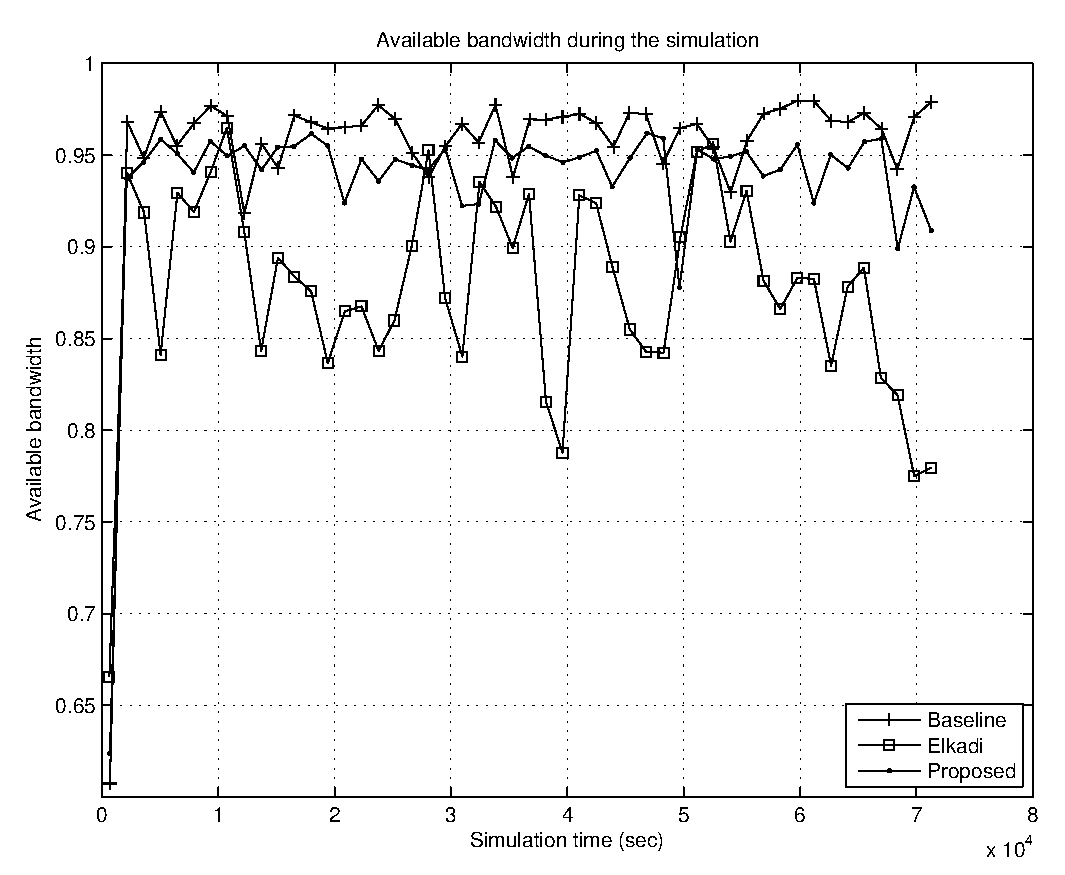
\includegraphics[width=4in] {clock_bs_availble_bw.eps}
\caption{基站的带宽利用率}\label{cacop_pic_clock_bs_availble_bw}
%\caption{Comparison of bandwidth utilization of a BS}\label{cacop_pic_clock_bs_availble_bw}
\end{figure}

%%%%%%%
%
\begin{figure}[htb]
\centering
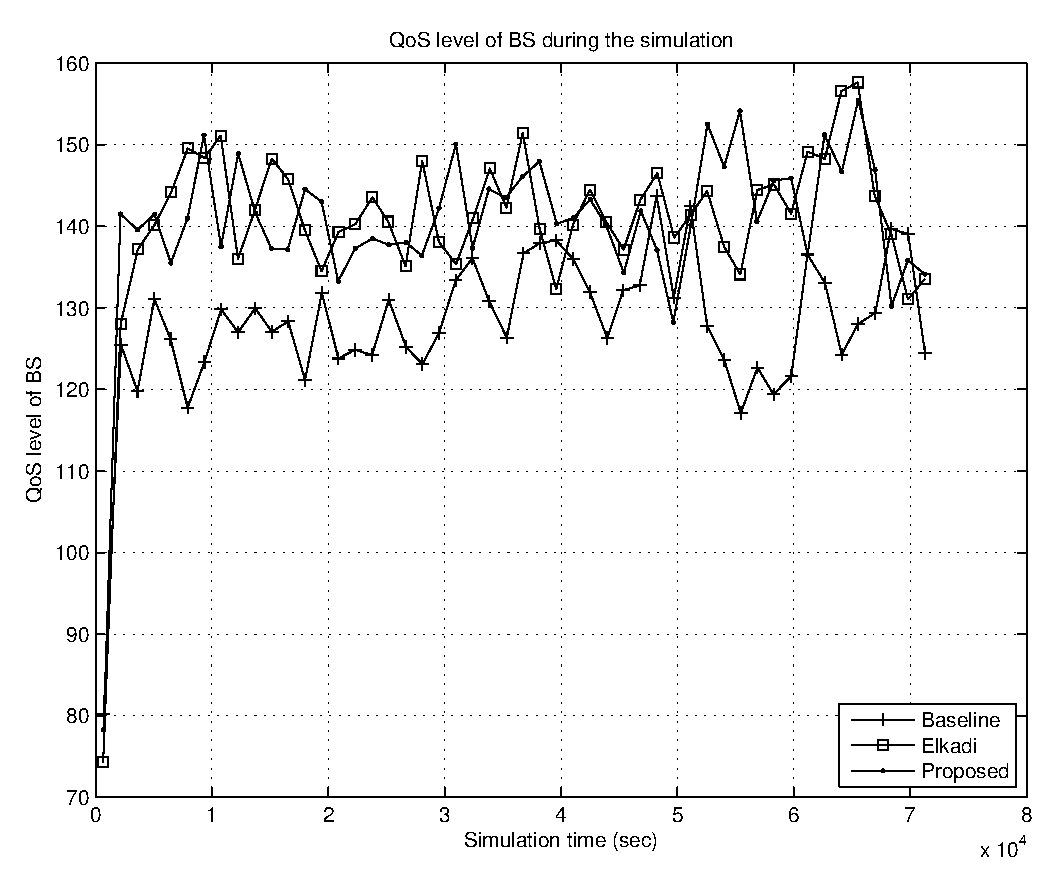
\includegraphics[width=4in] {clock_bs_qos_sum.eps}
\caption{基站的QoS水平}\label{cacop_pic_clock_bs_qos_sum}
%\caption{Comparison of QoS level of a BS}\label{cacop_pic_clock_bs_qos_sum}
\end{figure}

%%%%%%%
% 
\begin{figure}[htb]
\centering
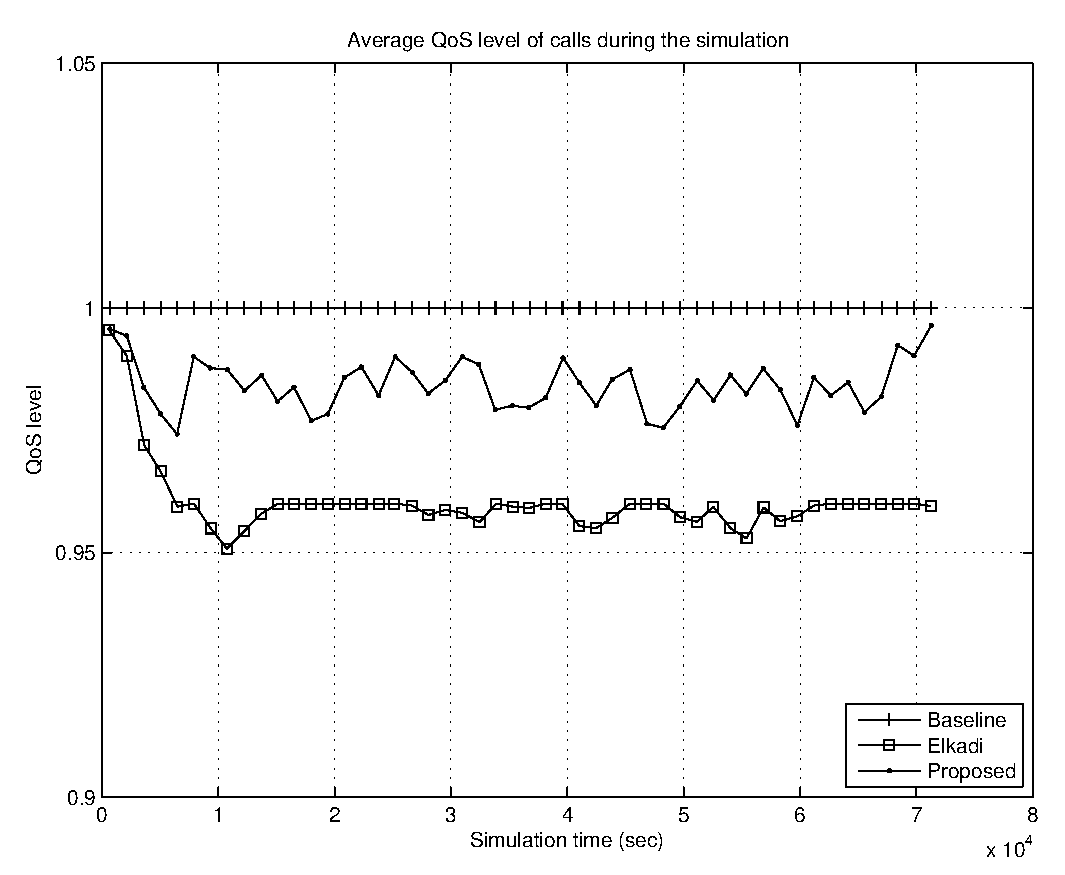
\includegraphics[width=4in] {clock_avg_call_qos.eps}
\caption{在线用户的平均QoS水平}\label{cacop_pic_clock_avg_call_qos}
%\caption{Comparison of average QoS level of connections}\label{cacop_pic_clock_avg_call_qos}
\end{figure}
\fi
%chapter_end
